\documentclass[11pt,a4paper,openright,twoside]{extreport}
\usepackage[utf8]{inputenc}
\usepackage[english]{babel}
\usepackage[inner=1cm,outer=1cm,top=2cm,bottom=2cm]{geometry}
\usepackage{amsmath}
\usepackage{amsfonts}
\usepackage{textcomp}
\usepackage{amssymb}
\usepackage{pifont}
\usepackage{epstopdf}
\usepackage[singlespacing]{setspace}
\usepackage{tabularx}
\usepackage{mathrsfs}
\usepackage{rotating}
\usepackage{caption}
\usepackage[usenames,dvipsnames]{xcolor}
\usepackage{fancyref}
\usepackage{subcaption}
\usepackage{braket}
\usepackage{color}
\usepackage{float}
\usepackage{enumerate}
\usepackage[pagebackref]{hyperref}
\usepackage{afterpage}
\usepackage[makeroom]{cancel}

% Start chapter on same page
\usepackage{etoolbox}
\makeatletter
\patchcmd{\chapter}{\if@openright\cleardoublepage\else\clearpage\fi}{}{}{}
\makeatother

\usepackage{fancyhdr}
\pagestyle{fancy}

\usepackage{graphicx}
\usepackage{subcaption}
\usepackage{wrapfig}
\graphicspath{{images/}}

\usepackage{todonotes}

\fancyhead{}
\fancyhead[RE, LO]{{\nouppercase{\leftmark}}}
\fancyhead[LE, RO]{\thepage}
\setlength{\headheight}{15pt}
\renewcommand{\headrulewidth}{0.4pt}

\fancyfoot{}
\fancyfoot[RE, LO]{{\nouppercase{{MAS-SS18 | Hochschule Bonn-Rhein-Sieg}}}}
\fancyfoot[LE, RO]{Dhole, Mensing, Padalkar}
\renewcommand{\footrulewidth}{0.4pt}

\hypersetup{
    pdftoolbar=true,        % show Acrobat’s toolbar?
    pdfmenubar=true,        % show Acrobat’s menu?
    pdffitwindow=false,     % window fit to page when opened
    pdfstartview={FitH},    % fits the width of the page to the window
    pdftitle={Scientific Experimentation and Evaluation Homework},    % title
    pdfauthor={Pranjal Dhole},     % author
    pdfsubject={Review},   % subject of the document
    pdfcreator={Pranjal Dhole},   % creator of the document
    pdfproducer={Pranjal Dhole}, % producer of the document
    pdfkeywords={SEEHomework} {Scientific Experimentation and Evaluation}, % list of keywords
    pdfnewwindow=true,      % links in new window
    colorlinks=true,       % false: boxed links; true: colored links
    linkcolor=MidnightBlue, % color of internal links (change box color with linkbordercolor)
    citecolor=Thistle,        % color of links to bibliography
    filecolor=magenta,      % color of file links
    urlcolor=Sepia           % color of external links
}

\newcommand{\sectionLine}{\begin{center}\line(1,0){500}\end{center}}
\definecolor{darkgreen}{RGB}{10, 127, 10}
\newcommand{\update}[1]{{\color{darkgreen}{#1}}}
%%%%%%%%%%%%%%%%%%%%%%%%%%%%%%%%%%%%%%%%%%%%%%%%%%%%%%%%%%%%%%%%%%%%%%%%%%%
%specific
\raggedbottom
%%%%%%%%%%%%%%%%%%%%%%%%%%%%%%%%%%%%%%%%%%%%%%%%%%%%%%%%%%%%%%%%%%%%%%%%%%%
\pagenumbering{arabic}
\begin{document}
%%%%%%%%%%%%%%%%%%%%%%%%%%%%%%%%%%%%%%%%%%%%%%%%%%%%%%%%%%%%%%%%%%%%%%%%%%%
\begin{center}
\section*{\underline{Scientific Experimentation and Evaluation}}
\large{\underline{Calibrating an Optical Tracking System}}\\
\large{Abhishek Padalkar, Max Mensing, Pranjal Dhole}\\
\large{Next submission: Thursday, 14$^{\text{th}}$ June, 2018}
\end{center}

\chapter{youBot placing experiment}
\section{Deliverables 6.1}
\textbf{Run the complete experiment with a KUKA youBot arm, i.e. run all 180 experimental trials and perform any necessary preprocessing of the data. You should submit a written report covering your observations, including appropriate figures. Your report should include:}

\subsection{Description of the experiment}

\begin{itemize}
	\item We were provided with a small, a medium and a large object.
	\item Each object has to be grasped and moved into 3 positions: Left, Right and Straight. The grasping, movement and release was pre-programmed.
	\item Each object has to be moved into each position 20 times.
	\item The following steps were repeated each time the experiment had to be performed:
	\begin{itemize}
		\item 1) Place the object on the marker on the table.
		\item 2) Grab the object using the arm.
		\item 3) Move the object to one of the 3 positions using the arm.
	\end{itemize}
	\item The measurements were recorded in a file for each measurement. Each file contained 50 JSON objects which were separated by lines counting the measurements.
	\item In order to extract the poses from this a python program was written to create clean CSV files which contain only the poses.
	\item Sorting of the files is handled by a bash script.
\end{itemize}


\subsection{Any observations made during the execution that may help to understand the outcome of the experiments; for instance, are there any particular sources of error that may affect the results of the experiment?}

\begin{itemize}
	\item In order to minimize all external sources of error, we have closed the curtains and used artificial light provided by the lamps at the ceiling.
	\item Since we measured vibrations in the table whenever the arm was moving we have only taken our measurements when the arm was not moving
	\item We did not move the chaird or walk while performing measurements since we were able to detect vibrations because of movement in the room
\end{itemize}

\subsection{A description of the pose filtering procedure you used and any observations that you may have made during the filtering process (e.g. on average, how many outliers are there per single experimental trial)}

\begin{itemize}
	\item For each run of the experiment a measurement was taken using the optical tracker.
	\item Each measurement recording consists of 50 pose recordings. This measurement redundancy is added to avoid measurement faults. The average of the 50 poses is taken as final pose for each measurement.
	
\end{itemize}


\subsection{The saved preprocessed data as Excel or LibreOffice Calc file or in a similar machine-readable form}

Those recordings have been saved in CSV files for each of the 3 experiments. They can be found in: \texttt{recordings/CSVs}.

\subsection{A visualization of the obtained final object poses. You are free to use any suitable visual representation for the data (using what you have already learned during the LEGO experiment). Hint: Given the different object-place combinations in the experiment, think about what we might want to illustrate with the visualization (e.g. the distribution of poses per object? the distribution of poses per motion direction? the distribution of all poses?)}


\begin{figure}[ht!]
	\centering
	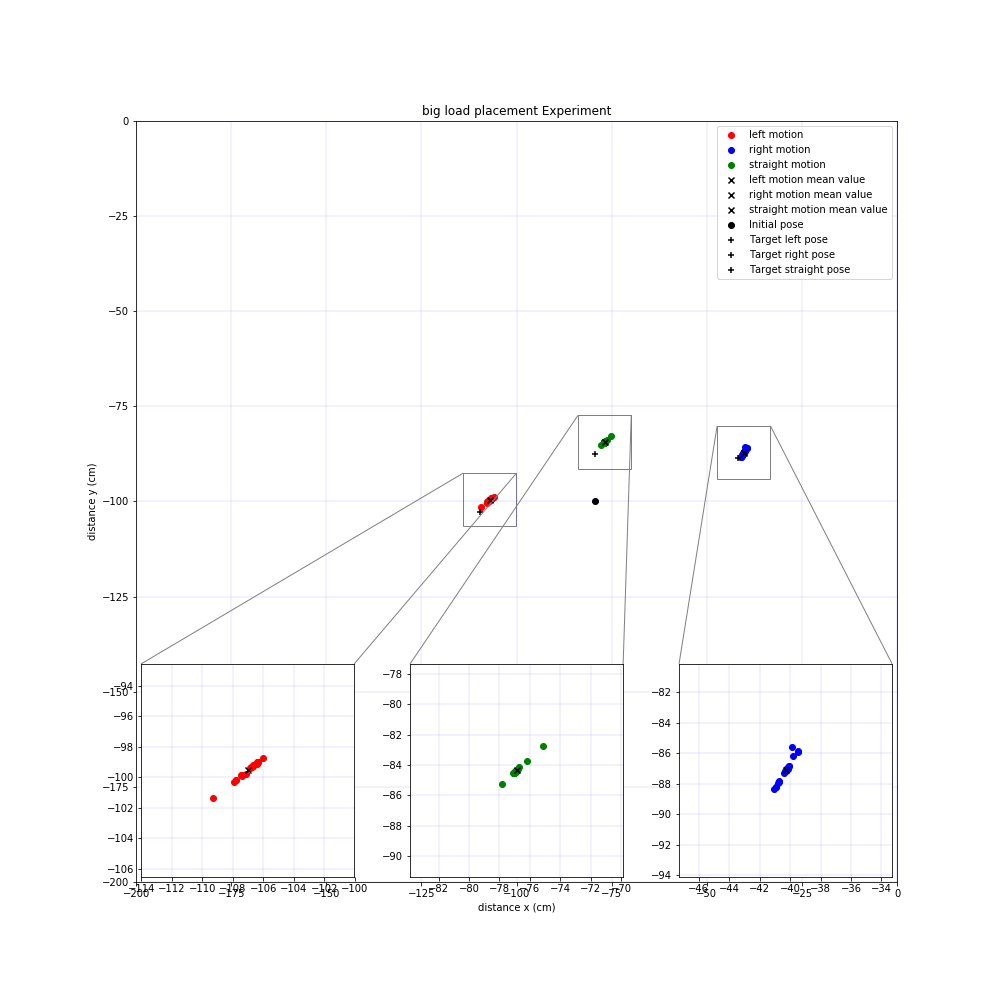
\includegraphics[width=0.6\linewidth]{images/big}
	\caption{Results of the Big Load Placement Experiment}
	\label{fig:big}
\end{figure}
\begin{figure}[ht!]
	\centering
	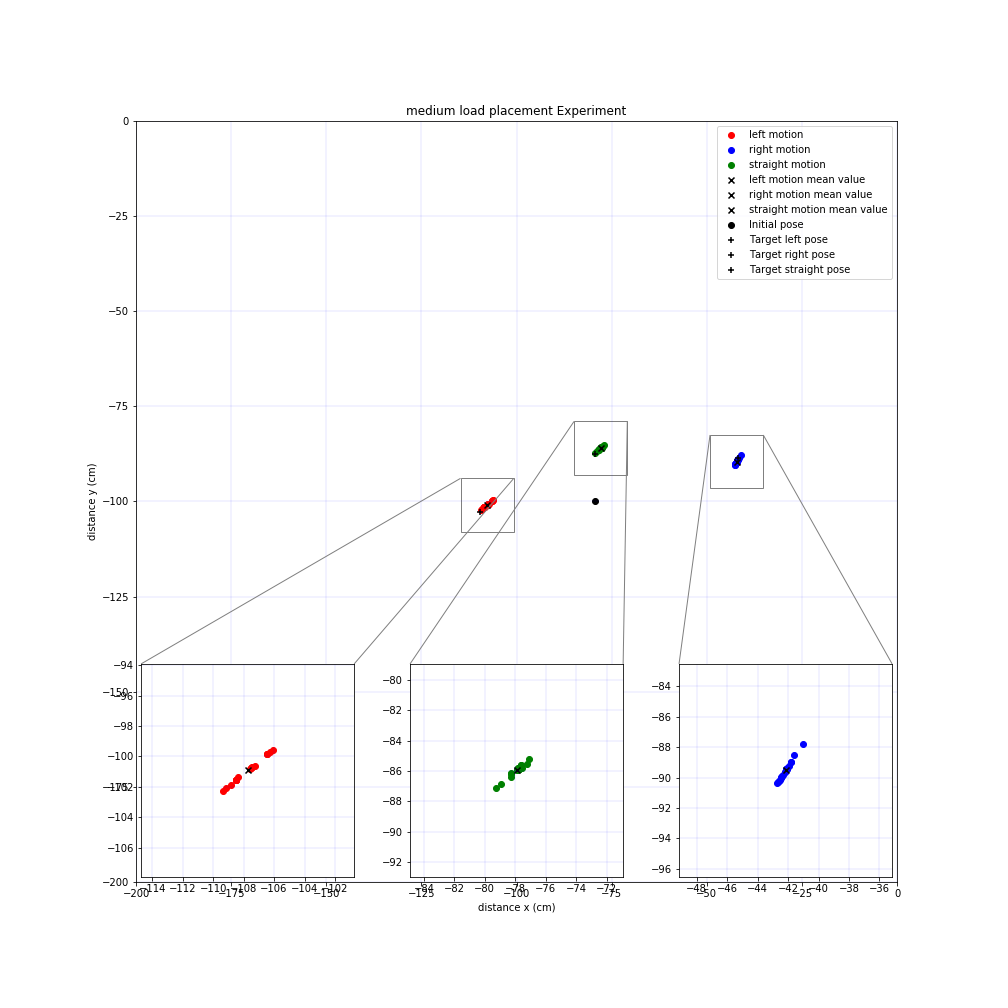
\includegraphics[width=0.6\linewidth]{images/medium}
	\caption{Results of the Medium Load Placement Experiment}
	\label{fig:medium}
\end{figure}
\begin{figure}[ht!]
	\centering
	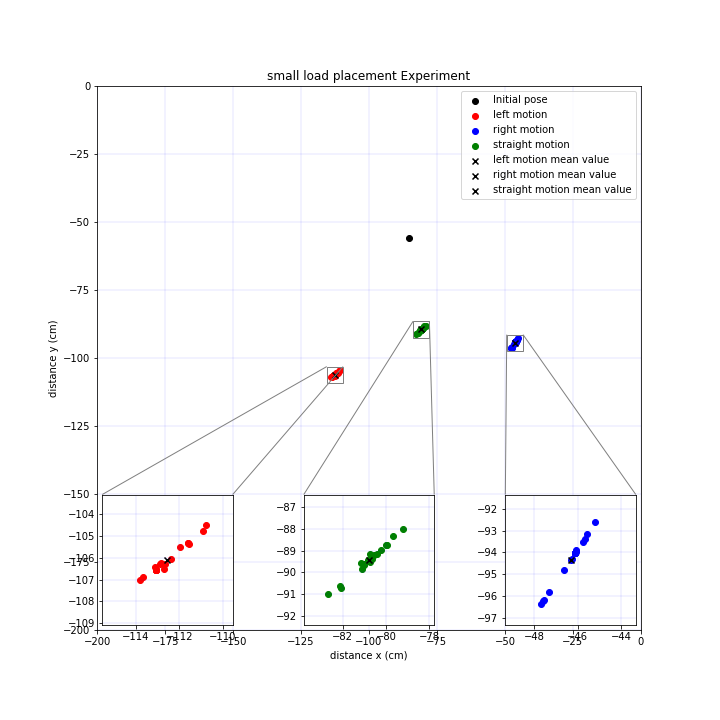
\includegraphics[width=0.6\linewidth]{images/small}
	\caption{Results of the Small Load Placement Experiment}
	\label{fig:small}
\end{figure}



\begin{figure}[ht!]
	\centering
	\begin{subfigure}[b]{0.3\textwidth}
		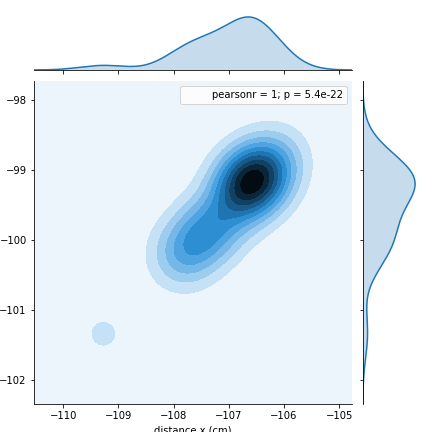
\includegraphics[width=\textwidth]{images/big_left.png}
		\caption{Left motion final pose.}
		\label{distribution-right-turn}
	\end{subfigure}
	\qquad
	\begin{subfigure}[b]{0.3\textwidth}
		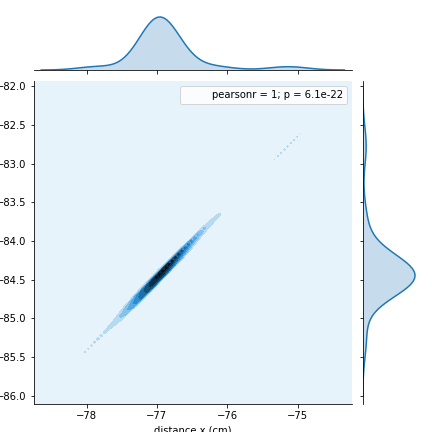
\includegraphics[width=\textwidth]{images/big_straight.png}
		\caption{Straight motion final pose.}
		\label{distribution-right-turn}
	\end{subfigure}
	\qquad
	\begin{subfigure}[b]{0.3\textwidth}
		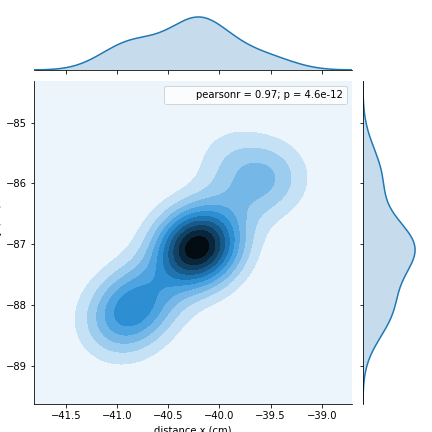
\includegraphics[width=\textwidth]{images/big_right.png}
		\caption{Right motion final pose.}
		\label{distribution-straight-motion}
	\end{subfigure}
	\caption{Gaussian and marginal distributions Final pose distribution - Big object}
\end{figure}

\begin{figure}[ht!]
	\centering
	\begin{subfigure}[b]{0.3\textwidth}
		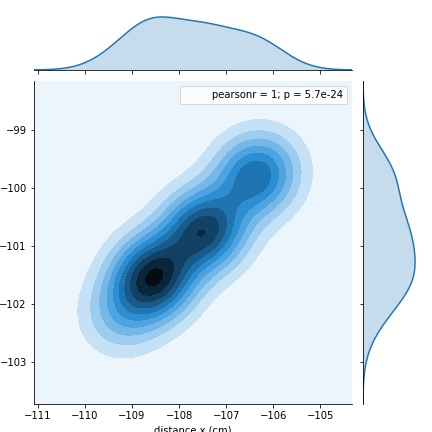
\includegraphics[width=\textwidth]{images/medium_left.png}
		\caption{Left motion final pose.}
		\label{distribution-right-turn}
	\end{subfigure}
	\qquad
	\begin{subfigure}[b]{0.3\textwidth}
		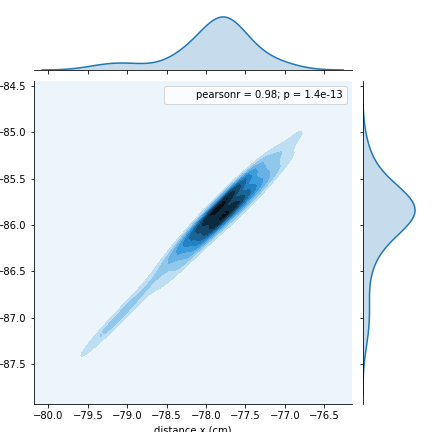
\includegraphics[width=\textwidth]{images/medium_straight.png}
		\caption{Straight motion final pose.}
		\label{distribution-right-turn}
	\end{subfigure}
	\qquad
	\begin{subfigure}[b]{0.3\textwidth}
		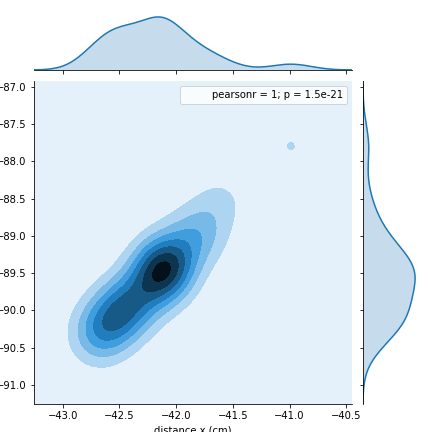
\includegraphics[width=\textwidth]{images/medium_right.png}
		\caption{Right motion final pose.}
		\label{distribution-straight-motion}
	\end{subfigure}
	\caption{Gaussian and marginal distributions Final pose distribution - Medium object}
\end{figure}

\begin{figure}[ht!]
	\centering
	\begin{subfigure}[b]{0.3\textwidth}
		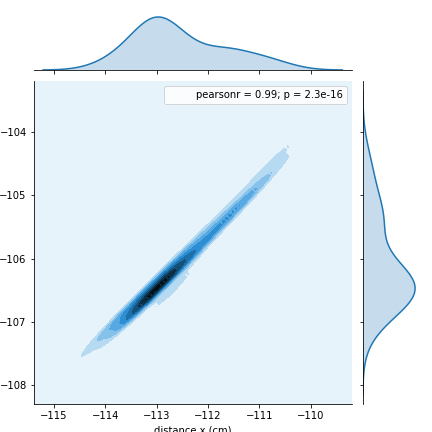
\includegraphics[width=\textwidth]{images/small_left.png}
		\caption{Left motion final pose.}
		\label{distribution-right-turn}
	\end{subfigure}
	\qquad
	\begin{subfigure}[b]{0.3\textwidth}
		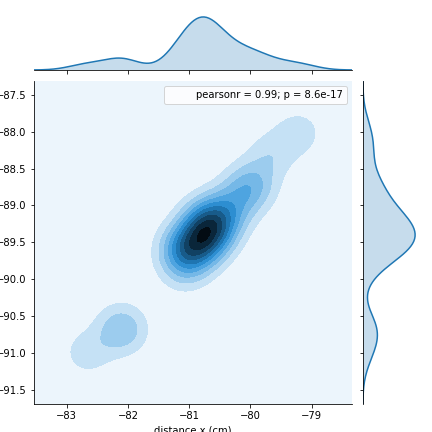
\includegraphics[width=\textwidth]{images/small_straight.png}
		\caption{Straight motion final pose.}
		\label{distribution-right-turn}
	\end{subfigure}
	\qquad
	\begin{subfigure}[b]{0.3\textwidth}
		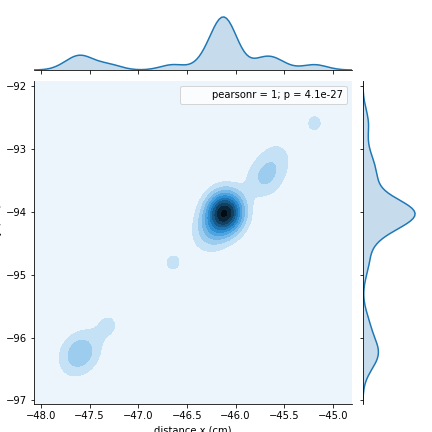
\includegraphics[width=\textwidth]{images/small_right.png}
		\caption{Right motion final pose.}
		\label{distribution-straight-motion}
	\end{subfigure}
	\caption{Gaussian and marginal distributions Final pose distribution - Small object}
\end{figure}


%%%%%%%%%%%%%%%%%%%%%%%%%%%%%%%%%%%%%%%%%%%%%%%%%%%%%%%%%%%%%%%%%%%%%%%%%%%%%
\section*{Assignment 1.2}
\subsection*{1. Robot configuration}
\label{robot-config}
\subsection*{2. Deliverables 1.2}
\subsubsection*{2.1 Robot design}
\textbf{Materials}
\begin{wrapfigure}{r}{0.4\textwidth}
  \vspace{-50pt}
  \begin{center}
    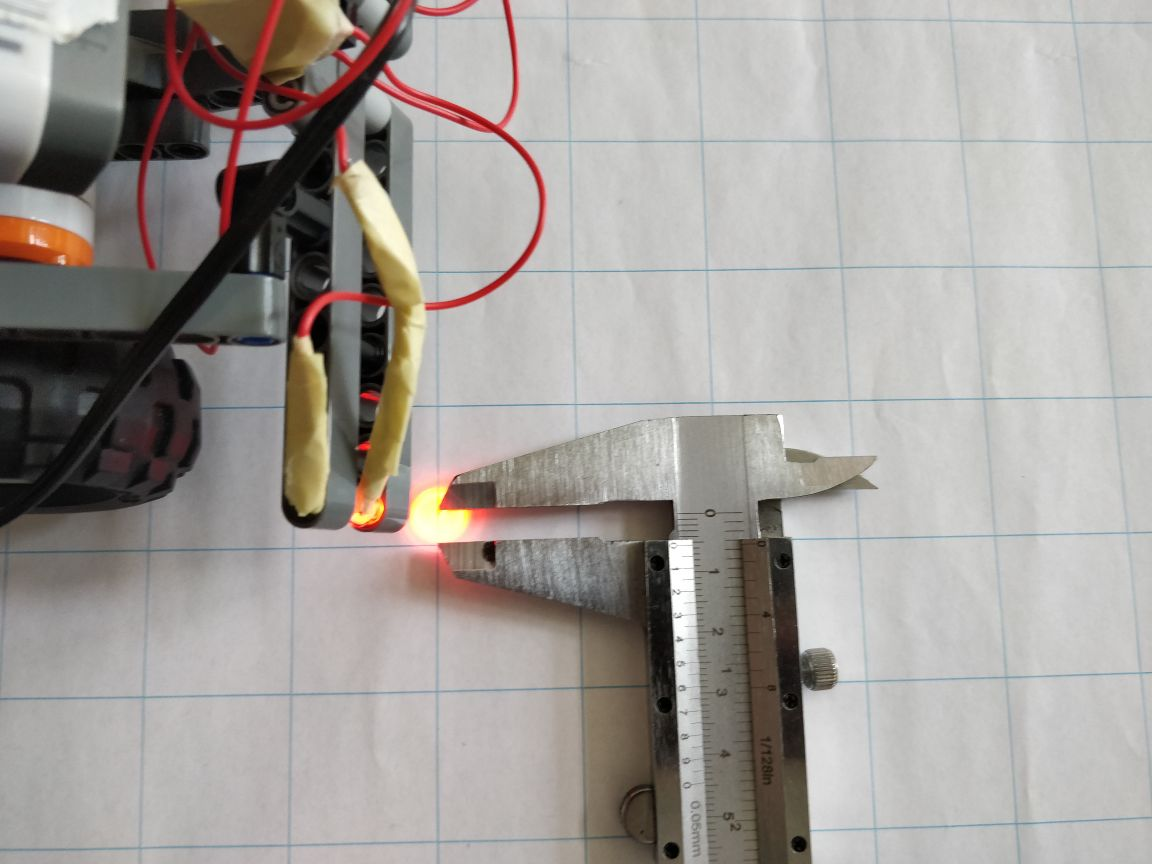
\includegraphics[width=0.39\textwidth]{fringe.jpeg}
  \end{center}
  \vspace{-20pt}
  \caption{Fringes formed on paper by LED lights.}
\end{wrapfigure}

We used the provided Lego Mindstorms 9797 toolkit for the construction of our robot.\\
The robot design is shown in the previous section.\\
For measurement purposes, we have mounted two LED lights with an approx. distance of $9.5 \pm 0.2$ cm in front of the Lego bot. \\
We have attached two resistors of 330 Ohms to each of the LEDs in order to reduce the current flowing through the LEDs. \\
The uncertainty is due to imprecise ruler measurements on each LED. The LED lights formed nice fringes on paper which made marking the center quite easy.\\
We use the provided  2.5x2.5cm grid paper for marking the positions of robot before and after each motion.\\
The corners of the grid paper were glued to the table in order to prevent an movement due to robot motion. 
\subsubsection*{2.2 Experiment}
\begin{itemize}
\item We run the LEGO NXT differential drive robot in three different configurations, viz., straight line motion, right turn motion and left turn motion.
\item The starting position of LEDs is marked on the grid paper and for each trial we align the centres of LED lights on the initial marked position on grid paper.
\item We collected 20 trial data of end robot positions for each configuration.
\item The observations made are tabulated in \texttt{motionData.csv} file attached.
\item The initial position for each configuration run is tabulated in \texttt{motionData\_init.csv} file.
\item In some of the trials the motion initiated in jerks which resulted in larger deviation. These points can be seen as extreme points from the mean of the distribution in each wheel data.
\item Another source of error is the orientation of the back wheel in the initial position. Since it is a passive castor wheel, this could have introduced some discrepancy in the motion.

\begin{figure}[H]
\centering
\begin{subfigure}[b]{0.49\textwidth}
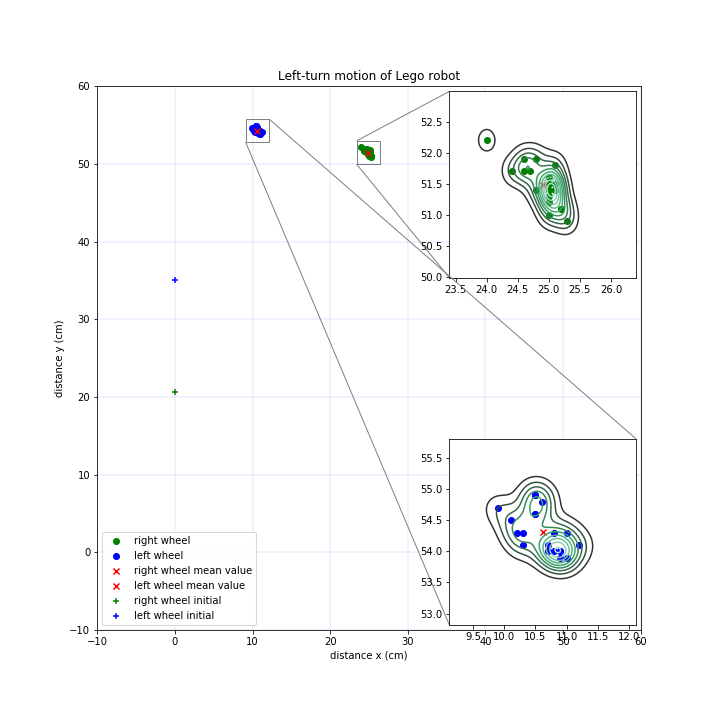
\includegraphics[width=\textwidth]{Left-turn.png}
\caption{Left turn motion}
\label{left}
\end{subfigure}
\begin{subfigure}[b]{0.49\textwidth}
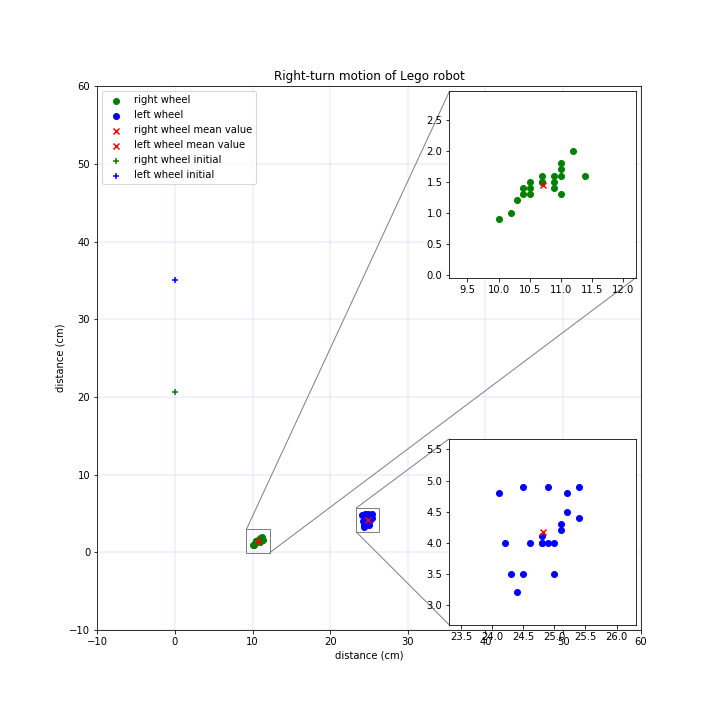
\includegraphics[width=\textwidth]{Right-turn.png}
\caption{Right turn motion}
\label{right}
\end{subfigure}
\begin{subfigure}[b]{0.49\textwidth}
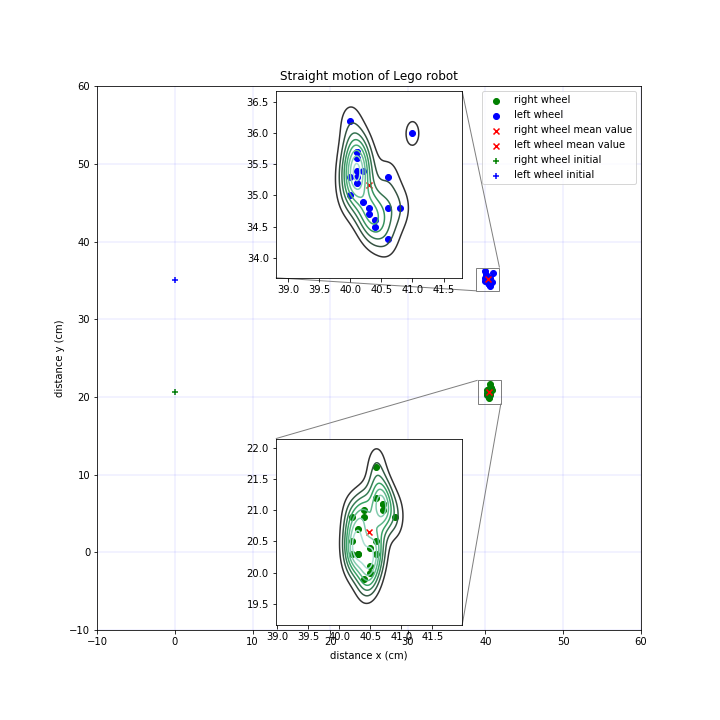
\includegraphics[width=\textwidth]{Straight.png}
\caption{Straight line motion}
\label{straight}
\end{subfigure}
\caption{Robot motion data. \update{x/y with units defined.}}
\label{data}
\end{figure}

\item In fig. \ref{data}, the robot motion data is visualized. The initial positions are marked by `+' sign and the mean positions are marked by `x' sign.

\item \textbf{Measurement error}: The accuracy of the position marker measurement due to unresolved LED center resolution was $\pm 1mm$.
\begin{table}[ht]
\centering
\begin{tabular}{| l | c | c | c | c | c | c |}
\hline
 & \multicolumn{2}{c|}{left-turn motion} & \multicolumn{2}{c|}{ right-turn motion} & \multicolumn{2}{c|}{straight motion} \\
\hline
 & right wheel & left wheel & right wheel & left wheel & right wheel & left wheel \\
\hline
Mean linear deviation $(\delta x, \delta y)$ cm & (0.1, 0.9) & (0.6, 0.8)
& (0.7, 0.9) & (0.2, 0.9) & (0.5, 0.4) & 0.3, 0.4) \\
\hline
Mean ang. deviation ($\delta \theta$) degrees & 0.9 & 2.3 & 2.7 & 1.1 & 0.6 & 0.6 \\
\hline
$\sigma$ in final pose (x,y) cm & (0.3, 0.3) & (0.3, 0.3) & (0.3, 0.2) & (0.4, 0.5) & (0.2, 0.5) & (0.3, 0.5)\\
\hline
uncertainty in pose (x) cm & $(0.1 \pm 0.3)$ & $(0.6 \pm 0.3)$ & $(0.7 \pm 0.3)$ & $(0.2 \pm 0.4)$ & $(0.5 \pm 0.2)$ & $(0.3 \pm 0.3)$ \\
uncertainty in pose (y) cm & $(0.9 \pm 0.3)$ & $(0.8 \pm 0.3)$ & $(0.9 \pm 0.2)$ & $(0.9 \pm 0.5)$ & $(0.4 \pm 0.5)$ & $(0.2 \pm 0.5)$ \\
\hline
\end{tabular}
\caption{Statistical summary of robot motion}
\label{stats}
\end{table}

\item In fig. \ref{left}, the standard deviation in readings of final wheel position for right and left wheels are (0.3, 0.3) cm and (0.3, 0.3) cm respectively.
\item In fig. \ref{right}, the standard deviation in readings of final wheel position for right and left wheels are (0.3, 0.2) cm and (0.4, 0.5) cm respectively.
\item In fig. \ref{straight}, the standard deviation in readings of final wheel positions for right and left wheels are (0.2, 0.5) cm and (0.3, 0.5) cm respectively.
\item This standard deviation is expected, since there is about 0.2 cm uncertainty in marking the end position of the robot as well as the initial jerky motion introduces some noise.
\item The standard deviations for left and right turn motions are very similar.
\item For straight line motion, we observe a substantial variation in y-readings.
\end{itemize}

%%%%%%%%%%%%%%%%%%%%%%%%%%%%%%%%%%%%%%%%%%%%%%%%%%%%%%%%%%%%%%%%%%%%%%%%%%%%%
%%%%%%%%%%%%%%%%%%%%%%%%%%%%%%%%%%%%%%%%%%%%%%%%%%%%%%%%%%%%%%%%%%%%%%%%%%%%%
\end{document}